\section{Contamination from Lensing}

We now consider gravitational lensing of the 21--cm signal by the large scale structure, as a source of noise in searches for magnetic fields using the method proposed in this work. We first compute the transverse shear power spectrum and then evaluate the bias it produces for the magnetic--field estimator. We demonstrate that this bias can be expected to be negligible, even for arrays with very futuristic collecting areas of $\sim 100$ km$^2$.

To follow standard lensing notation, we no longer label cartesian coordinate axes with $x$, $y$, and $z$, but rather with numbers, using the convention where directions $1$ and $2$ lie in the plane of the sky, while $3$ lies along the line of sight. Specifically, we use angular coordinates $(\theta_1, \theta_2)$ to denote direction in the sky ${\bf{\widehat n}}$, and $\theta_3$ to denote a comoving interval $r_z/\chi(z)$ along the line of sight, located at redshift $z$, and corresponding to $\Delta z$ interval. As before, we denote variables in Fourier space with tilde, and use $\vec{\ell}\equiv(\ell_1,\ell_2)$ for a conjugate variable of ${\bf{\widehat n}}$. 
 
We start by generalizing the formalism for two--dimensional weak lensing \cite{Weinberg201387} to the three--dimensional case.
In the presence of lensing, coordinate $\theta_i^S$, where $i\in\{1,2,3\}$, maps onto the observed coordinate $\theta_i$ as follows \begin{equation}
\theta_i^S=\theta_i+\frac{\partial\psi}{\partial\theta_i},\ i=1,2,3,
\label{eq:lensingmapping}
\end{equation}
where $\psi$ is the lensing potential. The full Jacobian of this coordinate transformation is
\begin{equation}
\frac{\partial\theta_i^S}{\partial\theta_j}=\delta_{ij}+\frac{\partial^2\psi}{\partial\theta_i\partial\theta_j}=(1+\kappa)I_{ij}+\gamma_{ij},\ \ \ i,j=1,2,3,
\label{eq:lensingtsf}
\end{equation}
where $I_{ij}$ represents the unity matrix. In the second step in the above Equation, we decomposed the symmetric $3\times 3$ matrix $\partial^2\psi/\partial\theta_i\partial\theta_j$ into a sum of a diagonal matrix and a symmetric traceless matrix $\bm{\gamma}$, representing magnification and shear, respectively. There are five independent shear components.
%The $\tilde{\gamma}_{13},\tilde{\gamma}_{23}$ components are the transverse shear components that we care about. Let's calculate the power spectrum of $\gamma_{13}$ first.

We now switch to Fourier space, where the two-dimensional Fourier transform of the lensing potential reads
\begin{equation}
\widetilde{\psi}(\vec{\ell},z)\equiv\int\psi({\bf\widehat{n}},z)e^{-i\vec{\ell}\cdot{\bf{\widehat n}}}\ d\theta_1 d\theta_2.
\label{eq:potentialFourier}
\end{equation}
The relation between $\psi$ and the Newtonian potential $\Phi$ in a flat universe is
\begin{equation}
\psi({\bf{\widehat n}},z)=
-2\int_0^{\chi(z)}d\chi_1\left[\frac{1}{\chi_1}-\frac{1}{\chi}\right]\Phi({\bf{\widehat n}},\chi_1),
\label{eq:lensingpotential}
\end{equation}
where $\chi_1$ is an integration variable.
Combining Eqs.~(\ref{eq:potentialFourier}) and (\ref{eq:lensingpotential}), we get 
\begin{equation}
\frac{\partial\widetilde{\psi}(\vec{\ell},z)}{\partial\theta_3}=-\frac{2}{\chi(z)}\int_0^{\chi(z)} d\chi_1\widetilde{\Phi}(\vec{\ell},\chi_1).
\label{eq:dpsi_dtheta3}
\end{equation}
From Eqs.~(\ref{eq:dpsi_dtheta3}) and (\ref{eq:lensingtsf}), it follows 
\begin{align}
&\langle\widetilde{\gamma}_{13}^*(\vec{\ell},z)\widetilde{\gamma}_{13}(\vec{\ell}',z')\rangle=\left\langle \ell_1\ell_1'\frac{\widetilde{\psi}^*(\vec{\ell},z)}{\partial\theta_3}\frac{\widetilde{\psi}(\vec{\ell}',z')}{\partial\theta_3}\right\rangle\nonumber\\
&=\frac{4\ell_1\ell_1'}{\chi(z)\chi(z')}\int_0^{\chi(z)}d\chi_1\int_0^{\chi(z')}d\chi_1'\langle\widetilde{\Phi}^*(\vec{\ell},\chi_1)\widetilde{\Phi}(\vec{\ell}',\chi_1')\rangle.
\end{align}

We now define the three--dimensional Fourier transform of the Newtonian potential $\widetilde{\widetilde\Phi}$ through
\begin{equation}
\widetilde{\Phi}(\vec{\ell},\chi)\equiv\int\widetilde{\widetilde{\Phi}}(\vec{\ell},\ell_3)e^{i\ell_3\chi}\frac{d\ell_3}{2\pi},
\end{equation}
where $\ell_3$ is an integration variabe. Using this definition, we get
\begin{align}
\langle\widetilde{\Phi}^*(\vec{\ell},\chi)\widetilde{\Phi}(\vec{\ell}',\chi')\rangle=\int\int&\frac{d\ell_3}{2\pi}\frac{d\ell_3'}{2\pi}\langle\widetilde{\widetilde{\Phi}}^*(\vec{\ell},\ell_3)\widetilde{\widetilde{\Phi}}(\vec{\ell}',\ell_3')\rangle\nonumber\\
&\times e^{i(\ell_3'\chi'-\ell_3\chi)}. \label{eq:doubletilde}
\end{align}
Assuming different modes are uncorrelated, we get
\begin{equation}
\bga
\langle\widetilde{\widetilde{\Phi}}^*(\vec{\ell},\ell_3)\widetilde{\widetilde{\Phi}}(\vec{\ell}',\ell_3')\rangle\\
=(2\pi)^3\delta(\ell_3-\ell_3')\delta^2(\vec{\ell}-\vec{\ell}')P_{\Phi}(\sqrt{\ell_3^2+\ell^2}).
\ega
\label{eq:expectation_tildetildephi}
\end{equation}
where
\begin{equation}
\bga
P_{\Phi}(\ell)=\frac{P_{\Phi}(k=\ell/\chi(z))}{\chi(z)^2}\\
=\left[\frac{3}{2}\Omega_mH_0^2(1+z)\right]^2\frac{P_{\delta}(k,z)}{k^4\chi(z)^2},
\ega
\end{equation}
is the angular power spectrum.
Substituting Eq.~(\ref{eq:expectation_tildetildephi}) into (\ref{eq:doubletilde}) and applying Limber approximation $\ell_3\ll\ell$, we obtain
\begin{equation}
\langle\widetilde{\Phi}^*(\vec{\ell},\chi)\widetilde{\Phi}(\vec{\ell}',\chi')\rangle=(2\pi)^2\delta^2(\vec{\ell}-\vec{\ell}')P_{\Phi}(\ell)\delta(\chi'-\chi),
\end{equation}
Thus, for $z\leq z'$,
\beq
\bga
\langle\widetilde{\gamma}_{13}^*(\vec{\ell},z)\widetilde{\gamma}_{13}(\vec{\ell}',z')\rangle\\
=\frac{4}{\chi(z)\chi(z')}\ell_1\ell_1'(2\pi)^2\delta^2(\vec{\ell}-\vec{\ell}')\int_0^{\chi(z)}d\chi_1P_{\Phi}(\ell).
\ega
\label{eq:exp_gamma13}
\eeq

We are interested in calculating the power spectrum $P_{13}(\vec{\ell},z,z')$ of $\gamma_{13}$ components, defined as
\begin{equation}
\bga
\langle\widetilde{\gamma}_{13}^*(\vec{\ell},z)\widetilde{\gamma}_{13}(\vec{\ell}',z')\rangle\equiv(2\pi)^2P_{13}(\vec{\ell},z,z')\delta^2(\vec{\ell}-\vec{\ell}').
\ega
\end{equation}
From Eq.~(\ref{eq:exp_gamma13}) we can express
\begin{equation}
P_{13}(\vec{\ell},z,z')=\frac{4\ell_1^2}{\chi(z)\chi(z')}\int_0^{\chi(z)}d\chi_1P_{\Phi}(\ell),
\end{equation}
where, as before, $\chi_1$ is an integration variable.
Similar result holds for the power spectrum $P_{23}$ of $\gamma_{23}$ component. Finally, the transverse power spectrum $P_t$ can be expressed as 
\beq
\bga
P_t(\ell,z,z')\equiv P_{13}+P_{23}\\
=\frac{4\ell^2}{\chi(z)\chi(z')}\int_0^{\chi(z)}d\chi_1P_{\Phi}(\ell).
\ega
\eeq
If $z=z'$, the above expression simplifies to
\begin{equation}
P_t(\ell,z)=\frac{4\ell^2}{\chi(z)^2}\int_0^{\chi(z)}d\chi_1P_{\Phi}(\ell).
\end{equation}
In Figure \ref{fig:Pt}, we show the transverse power spectra for a range of $z$, for standard cosmology.
\begin{figure}
\centering
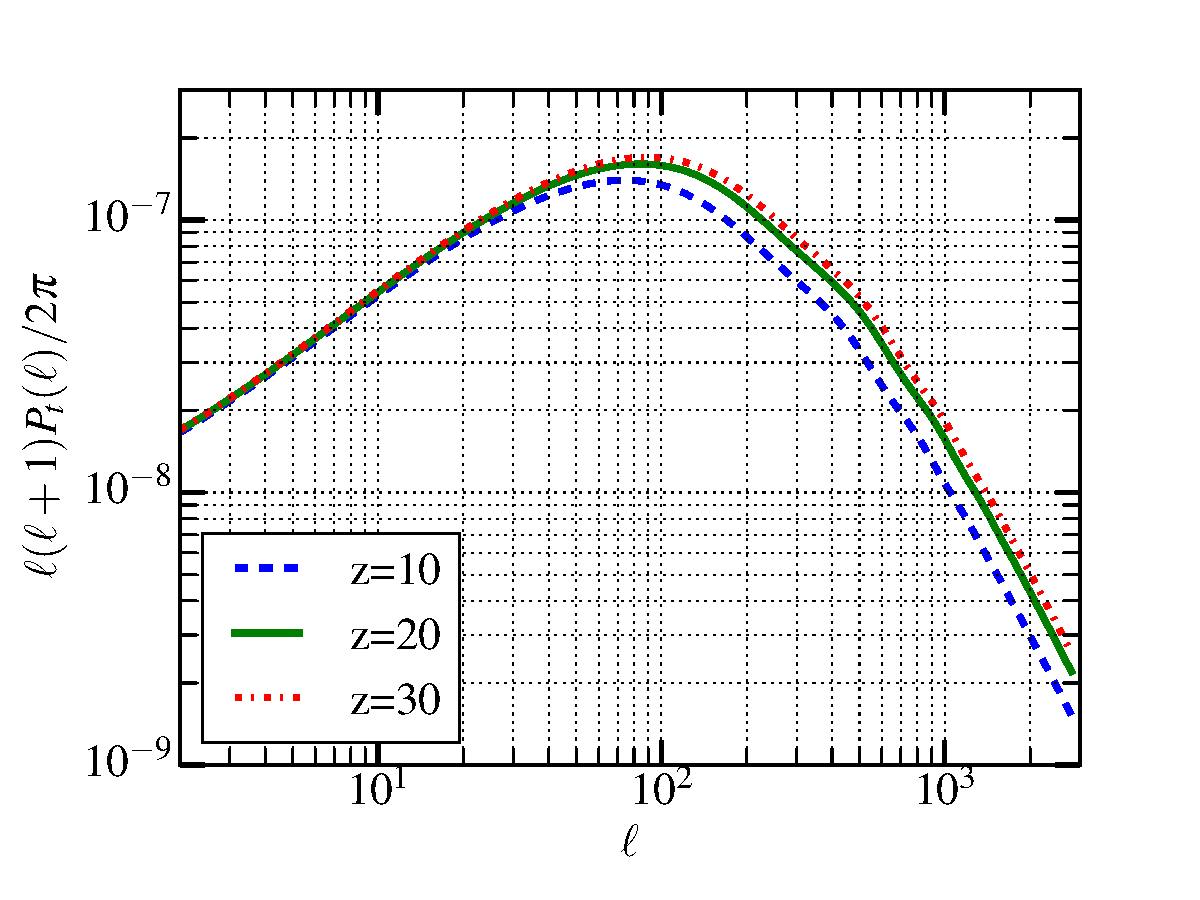
\includegraphics[scale=0.45]{lensing_transverse.pdf}
\caption{The transverse power spectra for sources at redshifts $z=10$, $20$ and $30$, computed for standard cosmology.}
\label{fig:Pt}
\end{figure}

Now that we have computed the transverse power spectrum $P_t$, we move on to evaluating the contamination it produces for the measurement of the magnetic field. We consider a configuration where the magnetic field is along the direction 2, ${\bf{\widehat k}}=(\sin\varphi,0,\cos\varphi)$, and the line of sight is along the direction 3, $\ {\bf{\widehat n}}=(0,0,1)$ in the three-dimensional Cartesian reference frame where $x$, $y$, and $z$ axes correspond to 3, 1, and 2, respectively; $\varphi$ is the angle between 3 and ${\bf{\widehat k}}$. Lensing distorts ${\bf{\widehat k}}$ and ${\bf{\widehat n}}$ into
\begin{align}
{\bf{\widehat k}}'&=\left(\begin{array}{c}
(1+\kappa+\gamma_{11})\sin\varphi+\gamma_{13}\cos\varphi\\
\gamma_{12}\sin\varphi+\gamma_{23}\cos\varphi\\
\gamma_{13}\sin\varphi+(1+\kappa+\gamma_{33})\cos\varphi
\end{array}\right),\nonumber\\
{\bf{\widehat n}}'&=\left(\begin{array}{c}
\gamma_{13}\\
\gamma_{23}\\
1+\kappa+\gamma_{33}
\end{array}\right),
\label{eq:distorted_kn}
\end{align}
and the shear only changes $\varphi$ by $-2\gamma_{13}$, to first order.
%The key to relating the shear effect to the magnetic fields is that the shear produces a similar precession of the quadrupole feature in the power spectrum of the brightness temperature. Since $P^S(\vec{k})=G^2({\bf{\widehat k}})P_\delta(k)$, the quadrupole feature can arise from both the transfer function and the lensed matter power spectrum. 

For conciseness, we define the coefficient $\bar{x}_{\rm B}\equiv x_{\rm B}/{B}$, and introduce the following short notation
\beq
\bga
%A&\equiv\left( 1 - \frac{T_\gamma}{T_{\rm s}} \right) x_{1{\rm s}} \left( \frac{1+z}{10} \right)^{1/2},\\
C\equiv0.128 \ {\rm mK} \left( \frac{T_\gamma}{T_{\rm s}} \right) x_{1{\rm s}} \left( \frac{1+z}{10} \right)^{1/2},\\
\mu_0\equiv 39.6-3C-\frac{C}{60}\frac{1}{1+x_{\alpha,(2)}+x_{c,(2)}},\\
\mu_1\equiv 13.2-C-\frac{C}{20}\frac{1}{1+x_{\alpha,(2)}+x_{c,(2)}},\\
\mu_2\equiv\frac{C}{10}\frac{x_B}{(1+x_{\alpha,(2)}+x_{c,(2)})^2}.
\ega
\eeq
For the configuration we chose, the transfer function in the presence of a small magnetic field reads
\beq
\bga
G^{(B)}=\left( 1 - \frac{T_\gamma}{T_{\rm s}} \right) x_{1{\rm s}} \left( \frac{1+z}{10} \right)^{1/2}\\
\times(\mu_0+\mu_1\cos 2\varphi+\mu_2\sin 2\varphi),
\ega
\eeq
where the $\sin 2\varphi$ term represents a precession of the emission quadrupole by a small angle $\epsilon$, in the sense that $\mu_1\cos 2\varphi+\mu_2\sin 2\varphi = \sqrt{\mu_1^2+\mu_2^2}\cos[2(\varphi+\epsilon)]$, where $2\epsilon\simeq\tan(2\epsilon)=-{\mu_2}/{\mu_1}$. Similarly, lensing also gives rise to $\sin 2\varphi$ term, such that
\beq
\bga
G^{(\text{lens, 13})}=\left( 1 - \frac{T_\gamma}{T_{\rm s}} \right) x_{1{\rm s}} \left( \frac{1+z}{10} \right)^{1/2}\\
\times \left[\mu_0+\mu_1(\cos 2\varphi+4\gamma_{13}\sin 2\varphi)\right].
\ega
\eeq
In addition, it affects the magnitude $k$, such that
\begin{equation}
k'=k(1+\kappa+\gamma_{11}\sin^2\varphi+\gamma_{33}\cos^2\varphi+2\gamma_{13}\sin\varphi\cos\varphi).
\end{equation}
to first order. Assuming $P_\delta(k)\propto k^{n_{\rm eff}}$, due solely to the lensing--shear $13$ component (and no magnetic field), we get
\beq
\bga
P^S(\vec{k}')=\left\vert G^{(\text{lens,
13})} \times (1+\kappa+\gamma_{11}\sin^2\varphi+\gamma_{33}\cos^2\varphi\right.\\
\left.+2\gamma_{13}\sin\varphi\cos\varphi)^{n_{\rm
eff}/2}\right\vert^2P_\delta(k)
\equiv \vert G'^{(\text{lens})}({\bf{\widehat k}'})\vert^2P_{\delta}(k).
\ega
\eeq
where $n_{\rm eff}$ is an effective spectral index (which is a function of the range of $k$ and redshift of interest; in our case, $n_{\rm eff}\sim -2.274$). Expanding $G'^{(\text{lens})}$, we find the $\sin 2\varphi$ term produced by the transverse lensing shear component, which mimics the precession effect due to the magnetic field, such that ${\mu_2}/{\mu_1}=\left[4+{n_{\rm eff}\mu_0}/({2}\mu_1)\right]\gamma_{13}$,
where we can solve for the spurious ``comoving magnetic field'',
\beq
\bga
B^{(\text{lens, 13})}=\frac{10(1+x_{\alpha,(2)}+x_{c,(2)})^2(4\mu_1+\frac{n_{\rm eff}}{2}\mu_0)}{C\bar{x}_{\rm B}(1+z)^2}\gamma_{13}\nonumber\\
\equiv\alpha\gamma_{13}.
\ega
\eeq
Finally, the lensing contamination to the magnetic--field reconstruction from $\gamma_{13}$ component is
\begin{equation}
P^{(\text{lens, 13})}(\ell)=\left\vert\frac{\partial B^{(\text{lens, 13})}}{\partial\gamma_{13}}\right\vert^2 P_{\gamma_{13}}(\ell)=\alpha^2 P_{\gamma_{13}}(\ell),
\end{equation}
while the total power spectrum gets an average value, i.e.~the half maximum,
\beq
P_B^{\rm lensing}(\ell)=\frac{\alpha^2}{2} P_t(\ell),
\eeq
and the root--mean--square (rms) of the total contamination is
\beq
\Delta^{(\text{lens})}(\ell)=\sqrt{\frac{\ell(\ell+1)}{2\pi}P^{(\text{lens})}(\ell)}.
\eeq
%Note that we only consider magnetic--field components perpendicular to the line of sight, where the shear contamination is maximized.  
We show numerical results for the rms contamination in Figure \ref{fig:lensing_B}, calculated with and without the de--lensing procedure (using CMB lensing measurements), with little difference found between the two cases. Comparing this result to Figure \ref{fig:Bsat}, we can see that the contamination due to lensing shear remains below the projected sensitivities even for the case of futuristic array sizes.
\begin{figure}[h]
\centering
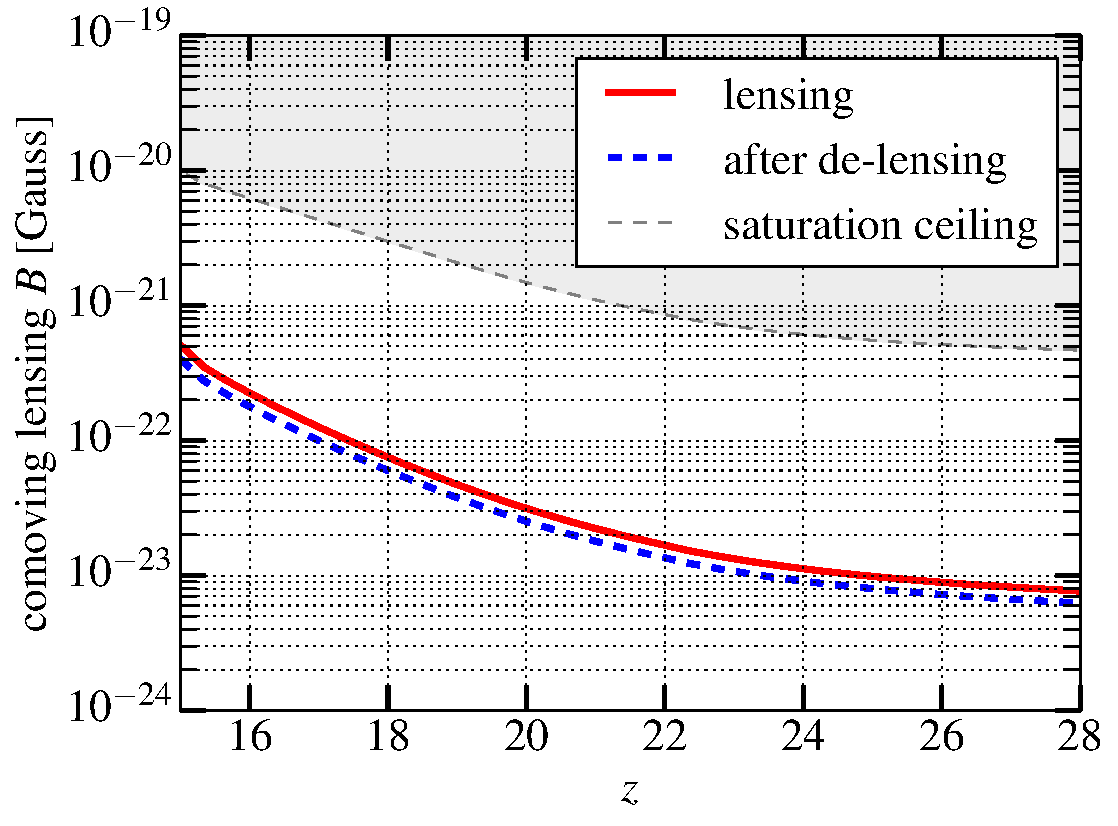
\includegraphics[scale=0.4]{delensingB.pdf}
\caption{Shown is the $1\sigma$ lensing--shear contamination to the measurement of the magnetic field, usind the method discussed in this work. Contamination before (solid red line) and after (dashed blue line) the de--lensing procedure, is presented as a function of redshift. Saturation ceiling is denoted by the shaded region above the thin dashed line. Comparison with Figure \ref{fig:Bsat} reveals that lensing is below the projected sensitivity for all array sizes considered in this work.}
\label{fig:lensing_B}
\end{figure}
%Finally, note that a survey of size $\Omega_{\rm survey}=1{\rm sr}$ corresponds to the scale of $\ell\sim6$, while the scale of the relevant matter fluctuations is determined by the resolution of the experiment from $k\sim \frac{2\pi L}{\lambda_0(1+z)D}\sim 1$, which corresponds to $n_{\rm eff}\sim -2.274$ in our case.

